\newcommand{\pararrow}[1]{
    \draw [->, thick] (-2,#1) -- (-0.5,#1);
}

\begin{center}
    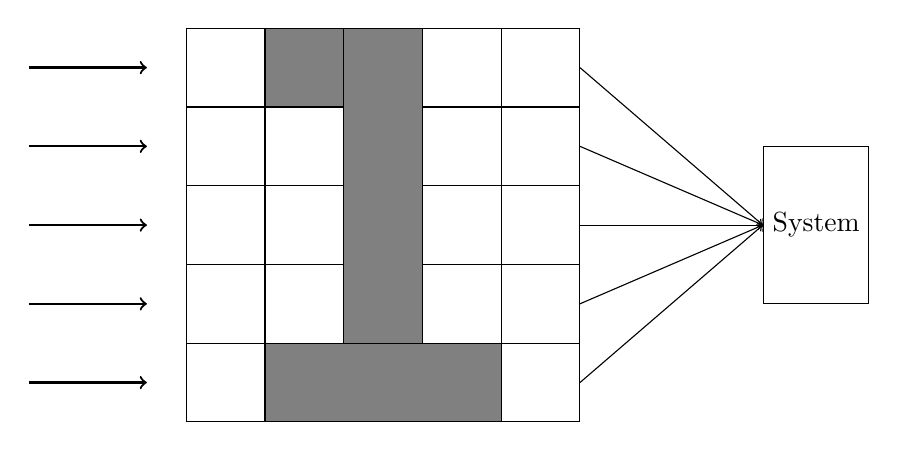
\begin{tikzpicture}
        \draw [step=1,black,thin] (0,0) grid (5,5);

        \draw [fill=gray] (2,0) rectangle (3,5);
        \draw [fill=gray] (1,0) rectangle (4,1);
        \draw [fill=gray] (1,4) rectangle (2,5);

        \node (system) at (8, 2.5) [draw, rectangle, minimum width=1cm, minimum height=2cm] {System};

        \uncover<2>{
            \pararrow{4.5};
            \draw [->] (5,4.5) -- (system.west);
        }
        \uncover<3>{
            \pararrow{3.5};
            \draw [->] (5,3.5) -- (system.west);
        }
        \uncover<4>{
            \pararrow{2.5};
            \draw [->] (5,2.5) -- (system.west);
        }
        \uncover<5>{
            \pararrow{1.5};
            \draw [->] (5,1.5) -- (system.west);
        }
        \uncover<6>{
            \pararrow{0.5};
            \draw [->] (5,0.5) -- (system.west);
        }

    \end{tikzpicture}
\end{center}